
%(BEGIN_QUESTION)
% Copyright 2003, Tony R. Kuphaldt, released under the Creative Commons Attribution License (v 1.0)
% This means you may do almost anything with this work of mine, so long as you give me proper credit

Safety is a paramount concern in electrical systems.  Generally, we try to design electrical circuits so that if and when they fail, they will do so in the manner safest to those people working around them, and to the equipment and process(es) controlled by the circuit.

One of the more common failure modes of circuits having wires strung through metal conduit is the {\it accidental ground}, or {\it ground fault}, where the electrical insulation surrounding a wire fails, resulting in contact between that wire and a grounded metal surface.

Suppose an accidental ground were to occur at the point shown in this ladder diagram:

$$\includegraphics[width=15.5cm]{i02313x01.eps}$$

What would be the result of this fault?  Hint: you will need to know something about the L1/L2 power source in order to answer this question!

What would be the result if the L1/L2 power connections were reversed?

\underbar{file i02313}
%(END_QUESTION)





%(BEGIN_ANSWER)

In a properly designed system, with L2 grounded at the power source, this fault will result in a blown fuse when the pressure switch closes.  In a circuit with L1 and L2 reversed, this same ground fault would energize the relief solenoid, with or without the pressure switch's ``permission.''

\vskip 10pt

Follow-up question: explain how a test instrument called a {\it megger} could be used to detect the presence of a ground fault.

%(END_ANSWER)





%(BEGIN_NOTES)

The ultimate purpose of this question is not to ascertain the effects of a particular fault so much as it is to derive a general rule regarding the construction of industrial control circuits.  Students should be able to see the benefits of having L2 (the grounded power rail) on the right-hand side of the circuit, but can they induce the general safety principle to be applied in all control circuits?  What is ``special'' about having L2 on the right-hand side of the ladder diagram?

%INDEX% Relay, diagram: ladder logic

%(END_NOTES)


